%part1.tex
\part{背景知识}

\section{简介}\label{sec:introduction}
当 Knuth 编写 \TeX\ 的时候,还没有 \prgname{PostScript}/\prgname{eps}、\prgname{jpeg}、\prgname{gif} 以及其它图像格式。
\marginpar{历史渊源}
因此 \prgname{dvi} 文件对于图像导入并没有直接的支持。
不过,\TeX{} 允许\file{dvi} 文件中包含 \cmd{spectial} 命令,
通过它可以向调用 \file{dvi} 文件的程序传递命令。
因此,凡是调用 \file{dvi} 的程序支持的图像格式,
\TeX\ 和 \LaTeX\ 都能够导入。

过去的许多年来,\file{dvi} 通常都被转为 \file{PostScript}格式,
进而标准的插图格式是 Encapsulated PostScript(\file{eps})图像,
因为它是PostScript语言的一个子集。
在 \LaTeX{} 中插入\file{eps}图像最初通过低层命令 \cmd{spectial} 来完成。
为了使插图更加方便并且更具有可移植性,
专门为 \LaTeX 2.09 设计了两个高层的宏包 \pkg{epsf} 和 \pkg{psfig}。
\textsf{epsf}~提供了 \cmd{epsfbox} 命令来插入图片,
此外另有三个命令来控制图片的缩放。
在 \pkg{psfig} 中,\cmd{psfig} 命令除了用来插入图片,还有缩放和旋转功能。
不过,尽管 \pkg{psfig} 的句法更受欢迎,它的代码却没有 \pkg{epsf} 健壮。
于是作为这两个宏包的结合的产物,
\pkg{epsfig} 宏包使用 \pkg{psfig} 的句法和大部分 \pkg{epsf} 的健壮代码。
不过,\pkg{epsfig} 仍然使用了一些不健壮的 \pkg{psfig} 代码。

随着 1994 年 \LaTeXe{} 的发布,\LaTeX 3 小组认识到在 \LaTeX{} 中插图的一些普遍问题。
\marginpar{\LaTeX{} 图形宏集}
通过努力,他们开发出了“\LaTeX\ 图形宏集”,
\footnote{已经有 \LaTeX{} 图形宏集的 plain \TeX{} 版本,
	相关文件请见 \href{ftp://ctan.tug.org/tex-archive/macros/plain/graphics/}{CTAN/macros/generic/graphics/}}
其中的命令全部重写。
比起其它的插入命令,他们的命令更高效、更健壮、更具有可移植性。

\LaTeX{} 图形宏集包括“标准”的 \pkg{graphics} 宏包和“扩展”的 \pkg{graphicx} 宏包。
这两个宏包都有一个 \cmd{includegraphis} 命令,不过版本不同。
类似 \pkg{psfig} 的句法,
\pkg{graphicx} 版的 \cmd{includegraphis} 采用“命名参数(named arguments)”。
这使用起来比较简单方便,却违反了 \LaTeX{} 关于可选参数放置位置的语法指南方针。
作为折中方案,就有了两种版本的 \cmd{includegraphis}。
其中,\pkg{graphics} 的版本遵从 \LaTeX{} 的语法规则,
而\pkg{graphicx} 的版本则采用更为简便的命名参数。
\pkg{graphicx} 版本的 \cmd{includegraphis} 支持图形的缩放和旋转,
而 \pkg{graphics} 版本的 \cmd{includegraphis} 则必须被置于 \cmd{scalebox} 或 \cmd{rotatebox} 才能达到同样的效果。

本文档使用 \pkg{graphicx} 宏包,因为它的句法比 \pkg{graphics} 宏包更加简便易用。
其实这两个宏包具有相同的功能,本文档中的例子同样可以用 \pkg{graphics} 宏包完成,
只不过相应的命令有些笨拙和缺少一点效率。
关于这两个宏包详细的说明可参见 \LaTeX{} 图形宏集的文档~\cite{grfguide}。

出于向后兼容性,\LaTeX\ 图形宏包套件中也提供了一个 \pkg{epsfig} 宏包,
用以替代之前 \LaTeXe\ 的 \pkg{epsfig}。
新的\pkg{epsfig} 定义了 \cmd{epsfbox}、\cmd{psfig} 和 \cmd{epsfig} 等命令。
不过它们只是调用 \cmd{includegraphics} 命令的简单封装。
由于这些封装效率没有直接使用 \cmd{includegraphics} 命令高,
因此,该 \pkg{epsfig} 宏包应当只用于旧文档。
在编写新文档时要用 \cmd{includegraphics}。

除了改进 \file{eps} 图片的部分,\LaTeX{}~图形宏集还处理非 \file{eps} 图像格式的插图问题,
例如\file{jpeg} 和 \file{gif}等。
\marginpar{非 \file{eps} 图形}
由于 \file{dvi} 到 \file{ps} 的转换程序一般不直接支持大部分的非\file{eps} 格式,
向 \file{PostScript} 文档中插入这些图像之前相关图像必须首先转成 \file{eps} 格式。
尽管这种图像格式的预处理通常是最佳办法,
不过,\LaTeX\ 图形宏集还提供了另一种选择:\file{dvi} 转 \file{ps} 时自动地实时转换图像格式。
第 \ref{ssec:convertor} 节(\pageref{ssec:convertor} 页)介绍了一下图像转换程序,
第 \ref{sec:noneps} 节(\pageref{sec:noneps} 页) 讲述了如何在 \file{dvi} 转 \file{ps} 时使用非 \file{eps} 格式的图像。

过去,\file{PostScript} 通常是 \LaTeX{} 文档的最终格式,
\marginpar{\pdfTeX}
整个编译过程有两个步骤:
(1) 使用 \LaTeX{} 生成 \file{dvi} 文件,
(2) 使用一个 \file{dvi} 到 \file{ps} 的转换程序(例如\prgname{dvips}) 来生成 \file{PostScript} 文件。
之后,随着 Adobe 的 \file{pdf} 格式开始流行,编译过程又加了第三步:
(3) 使用 \prgname{Ghostscript}
\footnote{自由软件,见第 \ref{ssec:ghostscript} 节(\pageref{ssec:ghostscript} 页)。}、
\prgname{Adobe Acrobat}
\footnote{商业软件,见 \url{www.adobe.com}}
或者 \prgname{PStill}
\footnote{共享软件,见 \url{www.pstill.com}}
等工具将 \file{PostScript} 文件转成 \file{pdf} 文件。

然而,这种三步骤过程 \LaTeX-\prgname{dvips}-\prgname{ghostscript} 不仅很繁琐,
而且很难实现一些 \file{pdf} 特性,比如超链接。
为了改进这一点,Hàn Thế Thành 写了一个工具叫做 \TeX2PDF,
这一工具修改了 \TeX\ 引擎,可以直接从 \TeX{} 生成 \file{pdf}。
\TeX2PDF 最终重命名为 \pdfTeX,
并且在许多志愿者的帮助下(托高德纳的福)进行扩展,
进而实现了 \TeX{} 的全部排版功能。
\pdfTeX 从名称上看来输出的是 \file{pdf},
不过它也能输出 \file{dvi} 格式,并且与原先 \TeX{} 引擎的输出结果相同。

如同 \prgname{latex} 命令使用 \TeX{} 处理 \LaTeX{} 文档来生成 \file{dvi} 文件,
\prgname{pdflatex} 命令使用 \pdfTeX{} 处理 \LaTeX{} 文档,并直接生成 \file{pdf} 文件。
 
\pdfTeX{} 的一个重要特性就是原生支持许多图像格式:
\marginpar{\pdfTeX{} 和图像}
\file{jpeg}、\file{png}、\file{pdf}、\file{MetaPost}。
尽管老版本的 \pdfTeX{} 还支持 \file{tiff} 文件,目前的 \pdfTeX{} 版本不支持 \file{tiff}。

另外要注意的是,\pdfTeX{} 不能直接导入 \file{eps} 文件
\footnote{\pdfTeX{} 可以导入由 \prgname{PurifyEPS} 处理的 \file{eps} 文件,
	见第 \ref{ssec:purifyeps} 节(\pageref{ssec:purifyeps} 页)。},
用户需要用 \prgname{epstopdf} 等程序将 \file{eps} 文件转成 \file{pdf} 格式,
不过这样就不能直接使用 PSfrag 宏包(见第 \ref{sec:psfrag} 节,\pageref{sec:psfrag} 页)。

\section{\LaTeX{} 术语}\label{sec:terminology}

任何 \LaTeX{} 对象(字符,图形等)都把\emphi{盒子}作为单位(\cite[page 103]{Leslie})。
每个盒子在它的左侧均有一个\emphi{参考点}(\emphi{Reference point})。
盒子的\emphi{基线}(\emphi{baseline},见图~\ref{fig:samplebox})是一条通过参考点的
一条水平线。
当 \LaTeX{} 从左到右排列文本时,
每一字符的参考点排成一条水平直线,称为\emphi{当前基线}(\emphi{current baseline}),
并使它与字符的基线对齐。
\LaTeX{} 也用同样的方法来处理图形和其它对象,每个对象的参考点都被放置于当前基线上。

\begin{figure}
	\centering
	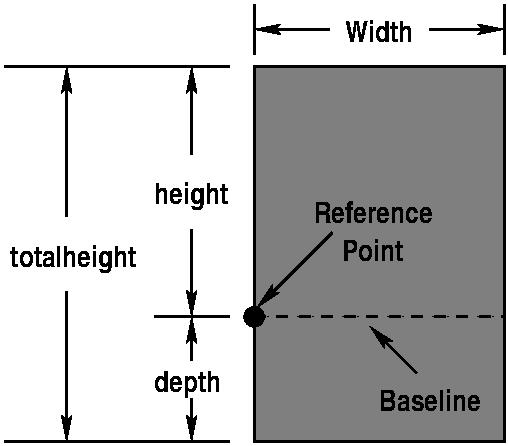
\includegraphics[width=.4\linewidth]{latex-box}
	\caption{\LaTeX{}~盒子示例}
	\label{fig:samplebox}
\end{figure}

每一个盒子的大小由三个长度决定:
\emphi{高度}(\emphi{height})、\emphi{深度}(\emphi{depth})和\emphi{宽度}(\emphi{width})。
高度是参考点到盒子顶部的距离,深度是参考点到盒子底部的距离,宽度则是盒子的宽度。
而\emphi{整体高度}(\emphi{totalheight})定义为盒子底部到顶部的距离,即
$\text{整体高度} = \text{高度} + \text{深度}$。

未旋转的 \file{eps} 图形的参考点是它的左下角(见图~\ref{fig:rotate-box}~的
左边的盒子),它的深度为零,高度就等于全部高度。
图~\ref{fig:rotate-box}~中间的盒子则是将图形旋转后,它的高度就不等于全部高度了。
右边的盒子则展示可将图形旋转使其高度为零。

\begin{figure}
	\centering
	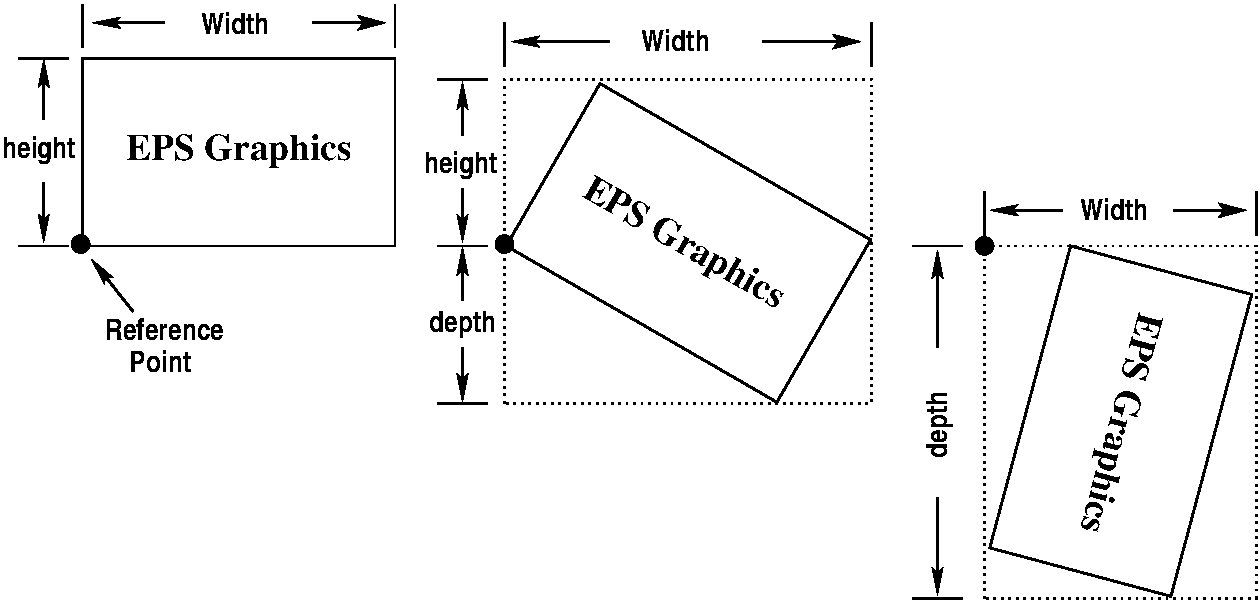
\includegraphics[width=.9\linewidth]{rotat-box}
	\caption{\LaTeX{}~盒子的旋转示例}\label{fig:rotate-box}
\end{figure}

\section{Encapsulated PostScript}\label{sec:eps}
PostScript 语言描述图像和文本。

PostScript 语言能够用来描述图形和文本。
它既可在传统的PostScript (\file{ps})文件中来描述多页文档,也用于 Encapsulated PostScript  (\file{eps})文件中来描述插入文档的图像。
\file{ps} 文件和 \file{eps} 文件的主要区别在于:
\begin{itemize}
	\item \file{eps} 文件只能使用部分特定的 PostScript 操作符。
	\item \file{eps} 文件必须含有一个~BoundingBox~行来确定 \file{eps} 图像的大小。
\end{itemize}


\subsection{禁止使用的 PostScript 操作符}\label{ssec:forbidps}

由于 \file{eps} 图形需要和其它对象一起共享页面,
所以~EPS~文件中不能使用页面操作,
例如选择页面大小(\texttt{a4}~或~\texttt{letter})和清除整个页面(\texttt{erasepage})等命令。
下面是不能在 \file{eps} 文件中使用的 PostScript 操作符:

\begin{center}
\ttfamily
\begin{tabular}{lllll}
	a3   &  a4 &  a5 &   banddevice & clear  \\
	cleardictstack & copypage &  erasepage & exitserver & framedevice \\
	grestoreall & initclip & initgraphics & initmatrix & letter  \\
	legal & note & prenderbands & quit & renderbands \\
	setdevice & setglobal & setpagedevice & setpageparams & setsccbatch \\
	setshared & startjob & stop & & \\
\end{tabular}
\end{center}

尽管下列 PostScript 操作符可以在 \file{eps} 文件中使用,
但是不适当地使用它们极易导致错误。
\begin{center}
\ttfamily
\begin{tabular}{llll}
	nulldevice & setcolortransfer & setgstate & sethalftone \\
	setmatrix & setscreen & settransfer & undefinedfont \\
\end{tabular}
\end{center}

上面的一些操作符可能会使\file{dvi} 到 \file{ps} 的转换失败,
另一些则可能导致像图像位置错误、消失或者闪烁等奇怪的问题。
因为这些操作符绝大部分不会影响到PostScript的堆栈,
所以在大多数情况下,简单地将这些招致问题的操作符删除就可解决问题。
其它的情形则需要更为复杂的PostScipt编程知识。

\subsection{The EPS BoundingBox}\label{ssec:bbox}
\index{EPS BoundingBox}

习惯上,PostScript 文件的第一行标明了该文件的PostScript类型,
接下来的几行是被称为 \emph{header} 或\emph{preamble} 的注释行(~PostScript 的注释符也是 \texttt{\%})。
其中一行定义了 BoundingBox,包括四个整数值,分别代表:
\begin{enumerate}
	\item BoundingBox 的左下角的 $x$ 坐标。
	\item BoundingBox 的左下角的 $y$ 坐标。
	\item BoundingBox 的右上角的 $x$ 坐标。
	\item BoundingBox 的右上角的 $y$ 坐标。
\end{enumerate}

例如,一个由 \prgname{gnuplot} 程序生成的 \file{eps} 文件的前五行为
\begin{Verbatim}[frame=single,rulecolor=\color{mygreen},label={\bfseries \file{eps} 文件头示例}]
%!PS-Adobe-2.0 EPSF-2.0
%%Creator: gnuplot
%%DocumentFonts: Times-Roman
%%BoundingBox: 50 50 410 302
%%EndComments
\end{Verbatim}

这个\prgname{gnuplot} 生成的 \file{eps} 图像的左下角的坐标是 $(50,50)$,
右上角的坐标是 $(410,302)$。
这里坐标的单位是PostScript 点,一点等于 $\nicefrac{1}{72}$ 英寸。
这样上面的这幅图的自然宽度为 $5$ 英寸,相应的自然高度为 $3.5$ 英寸。
需要注意的是PostScript 点要比 \TeX{} 点(等于 $\nicefrac{1}{72.27}$ 英寸)稍大。
在 \TeX{} 和 \LaTeX{} 中,PostScript 点被称为“大点”(``big points'')或简称 \texttt{bp},
而 \TeX{} 点被称为``points''或简称 \texttt{pt}。

\subsection{将PS转换为EPS}\label{ssec:pstoeps}

单页的PostScript文件,如果没有包含不适当的命令的话,
可用下述方法之一加上BoundingBox行并转为\file{eps}文件。
\textbf{由于这些方法都不检查非法的PostScript操作符,
	所以只有在被转换的PostScript文件本身不含有那些被禁制使用的操作符的情况下,才能得到正确的\file{eps} 文件。}

\begin{enumerate}
	\item 最方便的是用GhostScript里带的\prgname{ps2epsi}工具(见第~\ref{ssec:gs} 节,\pageref{ssec:gs} 页)。
	它可以读入PostScript文件,计算 BoundingBox 的参数,
	然后生成一个含有PostScript 图像的\file{eps} 文件。
	
	最终得到的 \file{eps} 文件是 \file{epsi} 格式,
	即它在文件的开始部分带有一个低分辨率的Interchange预览位图。
	因为这个预览位图是 \textsc{ASCII} 编码的,
	所以不会造成像第 \ref{ssec:linebuffer} 节的 \texttt{bufsize} 错误。
	不过,\file{epsi} 预览会增加文件体积。\index{bufsize@\texttt{bufsize}}
	\item 另外一种通过 Ghostscript 计算 BoundingBox 参数的方法是使用 \prgname{epstool} 工具。
	该程序适用于Unix、DOS、Windows和OS/2系统,获取链接为
	\begin{center}
		\url{http://www.cs.wisc.edu/ ~ ghost/gsview/epstool.htm}
	\end{center}
	例如,如下命令
\begin{verbatim}
    epstool --copy --bbox file1.eps file2.eps
\end{verbatim}
	分析 \file{file1.eps} 的内容来决定正确的 BoundingBox,
	然后将带有计算后的BoundingBox值的 \file{file1.eps} 内容复制给 \file{file2.eps}。
	\prgname{epstool} 工具还可以用于在 \file{eps} 文件内添加 \file{tiff}、\file{wmf} 以及 \file{epsi} 预览位图,
	或者用于从 \file{eps} 文件中提取预览位图。
	
	\item 此外,还有一种办法是,计算 BoundingBox 的参数,
	然后把它加到PostScript文件中或作为插图命令的参数
	(比如用 \cmd{includegraphics} 的 \texttt{bb} 选项)。
	计算BoundingBox 参数的方法有以下几种:	
	\begin{enumerate}
		\item 用 Ghostview 或 GSview 将 PostScript 图形打开。
		当鼠标在图形上移动时就会显示相应的坐标(以页面的左下角为参照点)。
		记下图形的左下角和右上角的坐标就可确定它的~BoundingBox。
		\item 将 PostScript 图形打印一份,
		测量页面的左下角到图像的左下角的水平和竖直距离(以英寸为单位),
		然后乘以 $72$ 就可以得到 BoundingBox 的左下角坐标。
		类似地,测量页面左下角到图像右上角的水平和竖直距离就可以得到 BoundingBox 的右上角坐标。
		\item \pkg{bbfig} 脚本使用 PostScript 打印机来计算 BoundingBox。
		\pkg{bbfig} 会在PostScript文件开头添加一些 PostScript 命令并送往PostScript打印机。
		在打印机处,添加的PostScript命令会计算 BoundingBox坐标,
		然后将结果打印在PostScript图像上面。
		\pkg{bbfig} 脚本程序的地址为
		\begin{center}
			\href{ftp://ctan.tug.org/tex-archive/support/bbfig/}{CTAN/support/bbfig/}
		\end{center}		
	\end{enumerate}
\end{enumerate}

\subsection{修正非标准的EPS文件}\label{ssec:fixeps}
一些应用程序(例如 \prgname{Mathematica} 和 \prgname{FrameMaker} )会生成非标准的 \file{eps} 文件,
不能在\LaTeX\ 等其它程序上使用。
有一些应用程序会根据它们自己的偏好给 PostScript 加入了额外特性,
还有一些应用程序生成非常糟糕的 PostScript 代码。
通常来说,这些非标准的PostScript可以由软件公司自己或者精通PostScript的用户提供的脚本来修正。
检索软件供应商的网页或者搜索相关软件的网络新闻组来获取相关信息。

\section{\LaTeX{} 怎样使用 EPS 图}\label{sec:useeps}

当处理\prgname{dvips} 类型文件时,\LaTeX{} 和 \file{dvi} 到 \file{ps} 的转换程序都会使用 \file{eps} 文件。
\begin{enumerate}
	\item \LaTeX{} 通过读取 \file{eps} 文件中的BoundingBox行来决定为 \file{eps} 图形保留多大的空间。
	\item \file{dvi} 到\file{ps}的转换程序读取\file{eps}文件并把它插入到生成的\file{ps} 文件中。
\end{enumerate}

需要说明的几种情形:
\begin{itemize}
	\item 如果在插图命令中给定了BoundingBox的值
	(例如,使用了 \cmd{includegraphics} 的 \opt{bb} 选项),
	\LaTeX{} 将不会再读取 \file{eps} 文件。
	事实上,当运行 \LaTeX{} 时,\file{eps} 文件甚至都不必存在。
	\item 由于 \TeX{} 不能读取非 \textsc{ascii} 文件,也不能生成其它的程序,
	所以 \LaTeX{} 不能从压缩的 \file{eps} 文件或其它非 \file{eps} 图像文件中得到BoundingBox的信息。
	在这种情况下,BoundingBox参数值必须由插图命令给定(例如 \cmd{includegraphics} 命令的 \opt{bb} 选项)
	或者存放在一个未压缩的文本文件中(见第~\ref{sec:noneps} 节,\pageref{sec:noneps}~页)。
	\item \file{eps} 图像并没有包含在\file{dvi}文件中。
	当 \file{dvi} 转换为 \file{ps} 时,\file{eps} 文件必须存在。
	因此,所有用到的\file{eps}文件必须和 \file{dvi} 文件放在一起。
	\item 一些 \file{dvi} 浏览器可能不支持显示 \file{eps} 图像。
	这时,为了方便使用者对图像进行定位,一般会将图形的BoundingBoX用一个方框显示出来。
\end{itemize}

\subsection[行缓冲区溢出]{行缓冲区溢出}\label{ssec:linebuffer}

\TeX{} 在读取 \textsc{ascii} 文件时是每次从中读取一行,然后把它放到自己的行缓冲区里。
\TeX{} 的行缓冲区大约有3000个字符长度。
如果 \file{eps} 文件中有一行的长度超过了行缓冲区的长度,就会产生如下的错误讯息:

\begin{Verbatim}[xleftmargin=22pt]
	Unable to read an entire line--bufsize=3000.
	Please ask a wizard to enlarge me.
\end{Verbatim}

因为\file{eps}很少有一行长度超过3000个字符的情形,
所以产生行缓冲区溢出错误的原因可能有两种:

\begin{enumerate}
	\item \textbf{ EPS 文件中有一个长的二进制预览图}

	有些应用程序生成的\file{eps} 文件在开始部分放置了一个二进制的预览图,
	这样就可使得像\file{dvi} 浏览器等一些不能解释PostScript的软件也可来显示 \file{eps} 图形。
	目前有少数与\TeX{} 有关的软件使用这种方法。
	
	如果这个二进制预览图比行缓冲区小,\cmd{includegraphics} 将会略过它
	\footnote{注意,\cmd{psfig} 和其它一些过时的图像命令则不会忽略二进制预览。}。
	但是,如果这个二进制的预览图比行缓冲区大的话,就会发生行缓冲区溢出的错误。
	对于该问题有两种解决办法:
	
	\begin{enumerate}
		\item 如果不需要预览图,可以用文本编辑器将它删掉或在一开始用应用程序生成\file{eps} 图像时就选择不要预览图。
		\item 因为 \LaTeX{} 读取 \file{eps} 文件的唯一目的就是取得BoundingBox参数值大小,、
		因此,如果插图命令中给出BoundingBox的值(如在 \cmd{includegraphics} 中使用 \opt{bb} 选项),
		那么\LaTeX{} 就不会读取 \file{eps} 文件。
	\end{enumerate}
	
	\item \textbf{\file{eps} 文件中的分行符在不适当的传输中被损坏}
	
	\emph{这里所谈到的问题不会在大部分最近的\TeX{} 发行版本中出现,
		因为这些软件中的\TeX{} 程序都会正确的识别所有的分行符。}
	
	不同的操作系统平台使用不同分行符。
	Unix 使用换行符LF(\verb+^J+),
	Macintosh 使用回车符CR( \verb+^M+),
	而 DOS/Windows 则使用回车符加换行符( \verb+^M^J+)。
	比如一个\file{eps} 文件从 Macintosh机上用二进制方式传输到Unix机上,
	那么Unix机上的\TeX{} 会因找不到分行符 \verb+^J+ 而把整个文件作为一行,导致行缓冲区溢出的错误。
	
	如果\file{eps} 文件中不含有二进制的部分(如预览图和嵌入的图形),
	以文本方式传输就可以解决这一问题。
	然而,带有二进制部分的 \file{eps} 文件必须用二进制方式传输,
	否则文本方式传输会损坏二进制部分。
	由于二进制传输方式不会翻译分行符,这时就需要在插图命令中给出BoundingBox的值来解决
	(例如\cmd{includegraphics} 命令的 \opt{bb} 选项)。
\end{enumerate}

\section{PDF 图像}\label{sec:pdfgraphics}
正如之前提到的,\pdfTeX{} 可以直接导入 \file{pdf}、\file{png}、\file{jpeg} 和 \file{MetaPost} 图像格式。
这一节将简要介绍这些格式。
相关的\pdfTeX{} 插图命令将在第~\ref{sec:graphicsinlusion} 节(\pageref{sec:graphicsinclusion} 页)中介绍。

\subsection{JPEG}\label{ssec:jpeg}
\file{jpeg} 是由联合图像专家组(Joint Photographic Experts Group , JPEG)委员会
\begin{center}
	\url{http://www.jpeg.org/}
\end{center}
授权的压缩标准。
\file{jpeg} 格式是一种位图的压缩标准,它采用了有损压缩格式
\footnote{有损压缩意味着压缩过程中损失了数据。
	也就是说,解压缩一个有损压缩过的位图不会得到原始图片。
	反之,无损压缩过程中不会有数据损失,
	所以解压一个无损压缩过的位图会生成原始图片。}。
特别地,压缩过程不会保持线条和锋锐的边缘。
所以不太适用于线条描绘和带有锋锐元素的图片。

\subsection{PNG}\label{ssec:png}
过去很多年 \file{gif} 一直是图标和其它线条画的位图压缩标准,
这是由于它采用的无损LZW压缩不会使得锋锐的边缘失真。
由于Unisys公司对于其LZW专利的强制执行,加上\file{gif} 的一些技术局限(例如256色的限制),
这些因素促使了一个小组开发可移植网络图形( Portable Network Graphics , PNG )格式。
该小组后来称为 \file{png} 开发组
\begin{center}
\url{http://www.libpng.org/pub/png/}
\end{center}
与 GIF 一样,PNG也采用无损压缩,因此适合于线条画。
尽管 \file{png} 可以用于任何位图文件,
不过对于摄影照片和其它一些没有锋锐边缘的位图来说,
\file{jpeg} 有损压缩通常效果更好( “更好”指的是生成更小的文件体积,同时对于人眼观察没有失真)。

\subsection{PDF}\label{ssec:pdf}
\href{http://www.adobe.com}{Adobe} 的便携式文档格式( Portable Document Format, pdf )与它的Adobe成员 PostScript 有很多相似之处。
与PostScript一样,\file{pdf} 可以包含文本、矢量图和位图。
一个 \file{pdf} 文件可以包含整个文档,也可以仅仅包含一个图形(类似于 \file{pdf} )。

\file{pdf} 不仅仅是 \pdfTeX{} 的主要输出格式,也是\pdfTeX{} 插图的最普遍方法。
许多图像程序允许它们的图像直接保存为 \file{pdf} 格式。
没有直接 \file{pdf} 输出的程序可以转而输出 \file{eps} 矢量图,
后者通过 \prgname{epstopdf} 转换程序可以很容易地转成 \file{pdf} 矢量图。
\prgname{epstopdf} 可以从 \textsc{ctan} 获得,
在Windows系统下是一个可执行程序,在Unix/Linux 以及 MaxOSX 等其它系统上则是一个\prgname{perl} 脚本
\begin{center}
\href{ftp://ctan.tug.org/tex-archive/support/epstopdf/}{CTAN/support/epstopdf/}
\end{center}

\subsection{MetaPost}\label{ssec:metapost}
MetaPost 是由John Hobby编写的绘图语言。
它基于高德纳的 \prgname{metafont},但增加了PostScript输出的功能。
关于MetaPost的信息可以从以下网址获得:
\begin{center}
\url{http://www.tug.org/metapost.html}\\
\url{http://cm.bell-labs.com/who/hobby/MetaPost.html}
\end{center}
相关文档可参考~\cite{MetaPost}。

MetaPost 可以用于 \prgname{dvips} 类型的 \LaTeX{} 文档,
也可以直接用于 \pdfLaTeX{} 文档\footnote{
	\pdfLaTeX{} 实际上使用Hans Hagen开发的 {Con\TeX t}代码将MetaPost图像实时转成 \file{pdf},
	不过在用户层面上是很简明的。}。

下面的步骤使用MetaPost( \prgname{mpost} )所带的 \prgname{pstoedit} 工具将名为 \file{graphic.eps} 的 \file{eps} 文件转为名为 \file{graphic.mps} 的 MetaPost 文件:

\begin{verbatim}
	pstoedit -f mpost graphic.eps graphic.mp
	mpost graphic.mp
	rename graphic.1 graphic.mps
\end{verbatim}

\subsection{PurifyEPS}\label{ssec:purifyeps}
Scott Pakin 的 \prgname{purifyeps} 工具能够将很多(但不是全部) \file{eps} 转成“净化版本”,
从而可以直接被 \LaTeX{} 和 \pdfLaTeX{} 读取。
为了运行 \prgname{purifyeps} 你需要下列工具:
\begin{description}
	\item[PurifyEPS] 可以从\href{ftp://ctan.tug.org/tex-archive/support/purifyeps/}{CTAN/support/purifyeps/} 获得,
	其中 \texttt{CTAN/} 使用第~\pageref{ctan-cite} 页中列出的任何\textsc{ctan} 站点替代。
	\item[Perl] 可以从 \url{http://www.cpan.org} 获得。
	\item[pstoedit] 可以从 \url{http://www.pstoedit.net/pstoedit} 获得。
	\item[mpost] 来自于任何包含MetaPost的\LaTeX{} 发行版本。
\end{description}


================================
\section[下载和安装\GS]{下载和安装~~\GS}\label{sec:gs}

\GS~是一个~\PS~语言解释器,它可以运行在大多数操作系统平台上并由~Aladdin
Enterprises~自由\realfootnote{Although Aladdin Ghostscript is distributed for
	free, it is not in the public domain. It is copyrighted and comes with
	certain limitations such as no commercial distribution. When versions of
	Aladdin Ghostscript become approximately one year old, Aladdin releases
	them as ``GNU Ghostscript'' whose use is governed by the less-restrictive
	GNU Public License.}发放。通过~\GS~可以在屏幕上显示~\PS~和~EPS~文件,也可
用非~\PS~打印机来打印。~Aladdin \GS~可从
~\href{ftp://ftp.ctan.tug/tex-archive/supported/ghostscript/aladdin/}%
{\texttt{CTAN/supported/ghostscript/aladdin/}}~取得。也可直接访问~\GS~的
主页:
\begin{quote}
	\href{http://www.cs.wisc.edu/~ghost/index.html}{\texttt{http://www.cs.wisc.edu/~ghost/index.html}}
\end{quote}
这一~Web~网址提供了比~CTAN FTP~站点更多更好的相关信息。
这些站点都提供~Windows/DOS/OS{\small /}2~和~Macintosh~的可执行文件,
~Unix/VMS~下的源代码。同时,还能下载~\GS~的图形用户界面(~Windows/OS/2~下
的~GSview~和~Unix/VMS~下的~Ghostview),这将使你更容易的观看和打印~\PS~文件。

Aladdin \GS~目前的正式版本为~6.01,~GNU \GS~的正式版本为~5.50。
对于~Window/DOS/OS{\small /}2~和~Macintosh~的用户来说,直接下载
它的已编译好的压缩包,安装使用就行了。而对于~Unix/VMS~的用户,通常
需要自己编译。编译时,首先将~\texttt{ghostscrip-x.xx.tar.gz}~和
其它所需的软件包解压缩:
\begin{Verbatim}[xleftmargin=1cm]
gzip -dc ghostscrip-x.xx.tar.gz | tar -vxf -
cd gsx.xx
gzip -dc ghostscrip-x.xxjpeg.tar.gz | tar -vxf -
gzip -dc ghostscrip-x.xxlibpng.tar.gz |tar -vxf -
gzip -dc ghostscrip-x.xxzlib.tar.gz | tar -vxf -
\end{Verbatim}
解压后可参考~GS~所带的帮助文件~make.txt~来按照你的要求编辑适当的~.mak~
文件,然后进行编译(假设使用~\texttt{gcc}~编译)和安装:
\begin{Verbatim}[xleftmargin=1cm]
ln -s src/gcc.mak ./Makefile
make
make install
\end{Verbatim}

\GS~中还带有一些有用的工具,如~\texttt{ps2pdf}~等,可利用~GS~来
转换图形,打印、预览~\PS~文件。详细的使用说明可参考~GS~所带的
使用说明文件。

\section{图像格式转换工具}\label{sec:convertor}

下面列出的一些免费软件和共享软件可以用来将非~EPS~格式的图形
转换为~EPS~图形。其中一部分提供命令行方式的软件,在用~\texttt{dvips}~
将~DVI~转为~PS~的过程中能同时自动转换图形的格式。具体见第~\ref{sec:noneps}~节。

\begin{itemize}
	\item \texttt{ImageMagick}~是一个很好的图形转换工具,可从
	~\href{ftp://ftp.wizards.dupont.com}{\texttt{ftp.wizards.dupont.com}}~或
	其它站点自由下载。参见:
	
	\href{http://www.wizards.dupont.com/cristy/ImageMagick.html}%
	{\texttt{http://www.wizards.dupont.com/cristy/ImageMagick.html}}
	
	除~Unix~和~Linux~外,它也可运行在~Windows NT, Macintosh~和~VMS~下。
	
	\item \texttt{xv}~是一个~\$25~的共享软件,运行在~X-Windows~环境下,可
	用来观看和转换图形。~\texttt{xv}~没有命令行方式,因此无法利用她来
	实现图形格式的即时转换功能。有关~\texttt{xv}~的信息可参见:
	
	\href{http://www.sun.com/sunsoft/catlink/xv/note.html}%
	{\texttt{http://www.sun.com/sunsoft/catlink/xv/note.html}}
	
	\texttt{xv}~的在线手册:
	
	\href{http://is.rice.edu/~shel/xv-3.10a/}{\texttt{http://is.rice.edu/~shel/xv-3.10a/}}
	
	\item \texttt{DISPLAY}~是~DOS~下的免费软件,能够转换多种图像格式。
	可从下面的地点下载~\texttt{disp189a.zip}~和~\texttt{disp189b.zip}~
	(新的版本可能不是~\texttt{189}~。)
	
	\href{http://www.simtel.net/simtel.net/msdos/graphics-pre.html}%
	{\texttt{http://www.simtel.net/simtel.net/msdos/graphics-pre.html}} \\
	\href{http://www.simtel.net/simtel.net/msdos/graphics-pre.html}%
	{\texttt{http://www.simtel.net/simtel.net/msdos/graphics-pre.html}}
	
	\item \texttt{WMF2EPS}~运行在~Windows9.x/NT~下的将~WMF~格式的图像转为~EPS~
	格式的免费软件。参考以下文件来取得这一软件。
	
	\href{ftp://ftp.tug.org/tex-archive/support/wmf2eps/readme.txt}%
	{\texttt{CTAN/support/wmf2eps/readme.txt}}
	
	它需要你的系统中装有~Adobe~兼容的打印机驱动。
	
	\item \texttt{KVEC}~是一个~\$25~的共享软件,能够将位图格式的图形(BMP, GIF,
	TIFF)等转为~\PS~或其它矢量图形。~\texttt{KVEC}~可运行在~Windows, OS/2,
	NEXT~和~Unix~下。
	
	\href{http://ourworld.compuserve.com/homepages/kkuhl/}%
	{\texttt{http://ourworld.compuserve.com/homepages/kkuhl/}}
	
	\item \texttt{NetPBM}~是旧有的~\texttt{PBMPLUS}~工具包的保留和扩充。
	目前它可运行在~Windows, Unix, VMS, DOS~等多种平台下。
	
	\href{http://wuarchive.wustl.edu/graphics/graphics/packages/NetPBM/}%
	{\texttt{http://wuarchive.wustl.edu/graphics/graphics/packages/NetPBM/}}
	
	\item \texttt{ImageCommander}~(共享软件,~\$19)是~Windows3.1/95/NT~下的
	图形转换软件,可将~GIF, JPEG, PICT, WMF~等多种图形转换为~EPS~和其它
	格式的图形。更详细的信息可见:
	
	\href{http://www.jasc.com/}{\texttt{http://www.jasc.com/}}
	
	JASC~的~Paint Shop Pro 绘图软件(共享软件,~\$69)具有同样的图形转换
	功能。
\end{itemize}

\subsection[Level 2 EPS~封装]{Level 2 EPS~封装}\label{ssec:epswrapper}

与传统的~\PS~不同的是,~Level 2 \PS~支持压缩的二进制图形。
这使得它能够制作出比传统的~EPS~更小、质量更好的图形。
如果你有一台~Level 2 \PS~打印机,那么你最好是用下面的
这些封装程序来替代上节中的那些转换软件。不过由于这样得到的~\PS~文件
只能在~Level 2 \PS~打印机上打印,会降低文件的通用性。

\begin{itemize}
	\item \texttt{jpeg2ps}~是一个用~C~语言程序,可将~JPEG~图形转换为~Level 2 \PS~
	图形。\texttt{jpeg2ps}~可在~Unix, DOS~和其它操作系统下使用。
	
	\href{http://www.muc.de/~tm/free/free.html}{\texttt{http://www.muc.de/~tm/free/free.html}}
	
	\item TIFF~图形可用~\texttt{tiff2ps}~转换为~LZW--编码的~Level 2 \PS~。
	\texttt{tiff2ps}~的源代码在:
	
	\href{ftp://ftp.sgi.com/graphics/tiff/tiff-v3.4-tar.gz}%
	{\texttt{ftp://ftp.sgi.com/graphics/tiff/tiff-v3.4-tar.gz}}
	
	\texttt{tiff2ps}~能在~Unix, DOS, Mac~和~VMS~下编译成功。尽管
	~LZW \PS~文件较小,但是它需要~~Level 2 \PS~打印机。
\end{itemize}

\subsection[编辑\PS]{编辑~~\PS}\label{ssec:editps}

虽然可直接编辑~EPS~文件中的~\PS~命令来改变图形,但这对一些不熟悉
~\PS~语言的人来说还是很困难的。所幸的是,借助于下面的一些工具软件,
可以很容易的编辑~EPS~图形。

\begin{itemize}
	\item \texttt{pstoedit} 是~Unix, Windows, DOS~和~OS/2~下的免费软件,
	借助于~\GS,它能购将~\PS~或~PDF~图形转为其它矢量格式(比如~
	\texttt{xfig}~的~\texttt{.fig}~格式)。~\texttt{pstoedit}~的
	C$++$~源码可从下述站点取得。
	
	\href{ftp://ftp.x.org/contrib/applications/pstoedit/pstoedit.html}%
	{\texttt{ftp://ftp.x.org/contrib/applications/pstoedit/pstoedit.html}}\\
	\href{http://www.geocities.com/SiliconValley/Network/1958/pstoedit/}%
	{\texttt{http://www.geocities.com/SiliconValley/Network/1958/pstoedit/}}
	
	\item \texttt{Mayura Draw}~(以前称为~\texttt{PageDraw})是~Windows3.1/9.x/NT~
	下的绘图软件。当与~\GS~一起使用时,它可以编辑~\PS~文件。见:
	
	\href{http://www.wix.com/PageDraw}{\texttt{http://www.wix.com/PageDraw}}
	
	旧版本的~\texttt{Mayura Draw}~是免费软件,最近的版本则为~\$15~的共享
	软件。~\texttt{Mayura Draw}~需要~Adobe Type Manager (ATM)~来在图形上
	放置文本。虽然~ATM~现在是商业软件,但是~Adobe~在~Acrobat Reader 2.0~中
	提供了一个免费版本。
	
	\href{ftp://ftp.winsite.com/pub/pc/win3/util/acroread.zip}%
	{\texttt{ftp://ftp.winsite.com/pub/pc/win3/util/acroread.zip}}
	
	\item \texttt{xfig}~是~Unix/Xwindows~下功能强大的免费绘图软件,能够
	引入~EPS~图形并加上标记。不过目前还不能改变原始的~EPS~图形。
	访问~\texttt{xfig}~的主页获取更进一步的信息。
	
	\href{http://www.xfig.org/}{\texttt{http://www.xfig.org/}}
	
\end{itemize}

\clearpage
\vbox to .5\textheight{\mbox{}}
\clearpage

\endinput
